\chapter{Graphen und Bäume}

% ===============
\section{Graphen}\label{sec_graphen}

\DEF Ein \emph{Graph}\index{Graph} $\GR$ besteht aus zwei Mengen
\begin{align*}
& E=E(\GR) \quad \text{(die \emph{Ecken}\index{Ecke} von $\GR$)} \\
& K=K(\GR) \quad \text{(die \emph{orientierten Kanten}\index{Kante}\index{orientierte Kanten}\index{Kante!orientiert} von $\GR$)}
\end{align*}
und den Abbildungen
\[
I : K \Ra E\times E,\quad k \mapsto (\ini(k),\ter(k))
\]
und
\[
\bar{\ }:K\Ra K,\quad k\mapsto\bar{k},
\]
mit den Eigenschaften
\begin{enumerate}
\item $k\neq \bar{k}$ für alle $k\in K$,
\item $\bar{\bar{k}}=k$ für alle $k\in K$,
\item $\ini(\bar{k})=\ter(k)$ für alle $k\in K$ (dann gilt auch $\ter(\bar{k})=\ini(k)$).
\end{enumerate}
Ein Paar $\{k,\bar{k}\}$ heißt \emph{geometrische Kante}\index{Kante!geometrisch}.

Mengenoperationen auf Graphen sind immer auf den entsprechenden
Mengen $E$ und $K$ zu verstehen.

\BSP Graphen.
\begin{center}
%	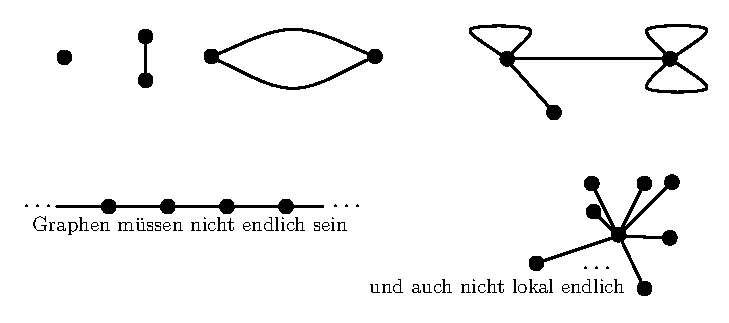
\includegraphics{bspgraphen}
\end{center}

\BEM $\GR$ kann \glqq topologisiert\grqq\ werden:
Geometrische Kanten werden mit $[0,1]$ identifiziert und verklebt,
wenn sie gemeinsame Ecken haben. Es ist sogar möglich, jeden
Graphen als Teilraum von $\RR^3$ zu realisieren, i.A. ist es aber nicht möglich, einen Graphen als Teilraum von $\RR^2$ zu realisieren
(siehe etwa Kapitel 3 in Diestel \cite{diestel}).

\DB Es seien $\GR=(E,K,I)$ und $\GR'=(E',K',I')$ Graphen.
\begin{enumerate}
\item Ein \emph{Morphismus}\index{Morphismus} $f:\GR\Ra\GR'$ ist ein
Paar $f=(f_E,f_K)$ von Abbildungen
$f_E:E\Ra E'$ und $f_K:K\Ra K'$ mit
\[
I'(f_K(k)) = ( f_E(\ini(k)), f_E(\ter(k)) )
= (f_E \times f_E)(I(k))
\]
und
\[
f_K(\bar{k}) = \bar{f_K(k)}
\]
für alle $k\in K$.
\item Die Komposition zweier Morphismen $f,g$
\[
f\circ g = (f_E\circ g_E, f_K\circ g_K),
\]
ist wieder ein Morphismus.
\item $f$ heißt \emph{Isomorphismus}\index{Isomorphismus}, wenn es
einen Morphismus $g:\GR'\Ra\GR$ gibt mit
\[
f\circ g = \id_{\GR'} \text{ und } g\circ f=\id_{\GR}.
\]
Ein Isomorphismus $f:\GR\Ra\GR$ heißt \emph{Automorphismus}\index{Automorphismus}.
\item $f$ ist genau dann ein Isomorphismus, wenn $f_E$ und $f_K$
bijektiv sind.
\end{enumerate}

\DB Es sei $\GR$ ein Graph.
\begin{enumerate}
\item Ein \emph{Weg}\index{Weg} $w$ (der Länge $|w|=n\geq 0$) in $\GR$
ist eine Folge
\[
w = (k_1,\ldots,k_n)
\]
von Kanten $k_i\in K$ mit $\ter(k_i)=\ini(k_{i+1})$ für
$i=1,\ldots,n-1$.
\[
\ini(w):=\ini(t_1) \text{ und } \ter(w):=\ter(k_n)
\]
heißen \emph{Anfangs-} und \emph{Endpunkt} von $w$.\index{Anfangspunkt}\index{Endpunkt}
Ist $n=0$, so wird $\ini(w)=\ter(w)\in E(\GR)$ definiert.
\item Setze
\begin{center}
%	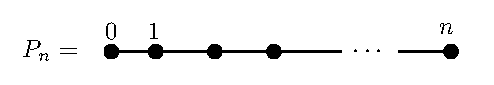
\includegraphics{Pn}
\end{center}
(fester Graph mit $n+1$ Ecken und $2n$ Kanten).
Dann ist jeder Weg der Länge $n$ in $\GR$ das Bild von $P_n$ unter
einem Morphismus $P_n\Ra \GR$.
\item $\GR$ heißt \emph{zusammenhängend}\index{zusammenhängend!Graph}\index{Graph!zusammenhängend},
wenn es für alle $x,y\in E$ einen Weg in $\GR$ gibt mit
$\ini(w)=x$ und $\ter(w)=y$.
\item Ein Weg heißt \emph{stachelfrei}\index{stachelfreier Weg}\index{Weg!stachelfrei},
wenn $k_{i+1}\neq \bar{k}_i$ ist für $i=1,\ldots,n-1$.
\item Gibt es in $\GR$ einen Weg von $x$ nach $y$, so gibt es auch
einen stachelfreien Weg.
\end{enumerate}
\textsc{Beweis von 5.:} Es sei $w=(k_1,\ldots,k_n)$ und
$k_{i+1}=\bar{k}_i$. Dann gilt:
\[
\ini(k_{i+2}) = \ter(k_{i+1}) = \ter(\bar{k}_{i})
= \ini(k_i) = \ter(k_{i-1}).
\]
Folglich ist $w'=(k_1,\ldots,k_{i-1},k_{i+2},\ldots,k_n)$ ein
Weg von $x$ nach $y$.
\qed

\DB Es sei $\GR$ ein Graph.
\begin{enumerate}
\item Ein Weg $w$ in $\GR$ heißt \emph{geschlossen}\index{geschlossener Weg}\index{Weg!geschlossen},
wenn $\ini(w)=\ter(w)$.
\item $w$ heißt \emph{einfach}\index{einfacher Weg}\index{Weg!einfach},
wenn $\ini(k_i)\neq\ini(k_j)$ für $i\neq j$.
\item Einfache Wege sind insbesondere auch stachelfrei (für Wege
der Länge $2$ ist dies als Definition zu verstehen).
\item Ein einfacher geschlossener Weg der Länge $n\geq 1$ heißt
\emph{Kreis}\index{Kreis}\index{Weg!Kreis}.
Ein Kreis der Länge $1$ heißt \emph{Schleife}\index{Schleife}\index{Weg!Schleife}\index{Kreis!Schleife}.
\begin{center}
%	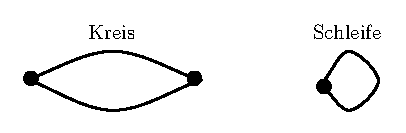
\includegraphics{kreis}
\end{center}
\item Ein Paar $k_1\neq k_2$ von Kanten in $\GR$ heißt \emph{Doppelkante}\index{Doppelkante}\index{Kante!Doppel-},
wenn $\ini(k_1)=\ini(k_2)$ und $\ter(k_1)=\ter(k_2)$ ist.
\begin{center}
%	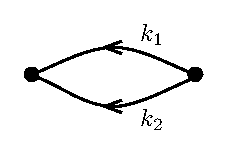
\includegraphics{doppelkante}
\end{center}
\item Ein Graph heißt \emph{kombinatorisch}\index{kombinatorischer Graph}\index{Graph!kombinatorisch},
wenn er keine Schleifen und keine Doppelkanten enthält.
\item Ein Graph ist genau dann kombinatorisch, wenn er als
topologischer Raum ein simplizialer Komplex ist.\index{simplizialer Komplex}
\end{enumerate}

\DB Es sei $\GR$ ein zusammenhängender Graph. Für $x,y\in E$ sei
\[
d(x,y) := \min\{ n : \text{ es gibt einen Weg $w$ von $x$ nach $y$
	mit $|w|=n$} \}.
\]
Dann ist $d$ eine Metrik auf $\GR$ (genauer: auf $E(\GR)$).
Der \emph{Durchmesser}\index{Durchmesser} von $\GR$ ist
\[
d(\GR) := \sup\{ d(x,y) : x,y\in E\}.
\]

%==============================
\section{Bäume}\label{sec_baum}

\DEF Ein \emph{Baum}\index{Baum}\index{Graph!Baum} ist ein
zusammenhängender Graph ohne Kreise.

\BSP Bäume.
\begin{center}
%	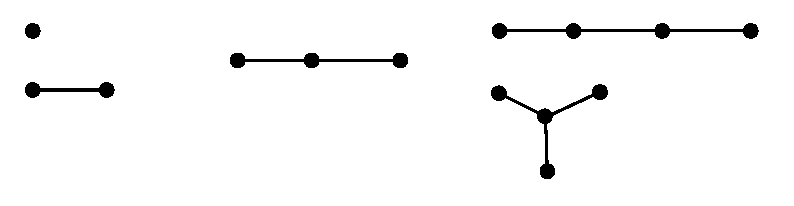
\includegraphics{bspbaum}
\end{center}

\PROP Ein Graph $\GR$ ist genau dann ein Baum, wenn es zu je zwei
seiner Ecken $x,y$ einen stachelfreien Weg von $x$ nach $y$ in
$\GR$ gibt.

\bew \glqq$\ra$\grqq: Seien $x,y\in E(\GR)$,
$w=(k_1,\ldots,k_n)$ und $w'=(k'_1,\ldots,k'_m)$ stachelfreie Wege
von $x$ nach $y$. Ist $k_n\neq k'_m$, so ist
$\tilde{w}=(k_1,\ldots,k_n,\bar{k}'_m,\ldots,\bar{k}'_1)$
ein stachelfreier geschlossener Weg, enthält also einen
Kreis, im Widerspruch dazu, dass $\GR$ ein Baum ist.
Also muss $k_n=k'_m$ sein. Induktion über die Weglänge $n$ ergibt
die Behauptung.

\glqq $\la$\grqq: Da es zwischen je zwei Ecken einen Weg gibt, ist
$\GR$ zusammenhängend. Da es genau einen Weg gibt, kann es keine
Kreise geben.
\qed

\DB Sei $\GR$ ein Graph und $x\in E(\GR)$.
\begin{enumerate}
\item Es sei
\[
K_x := \{ k\in K(\GR) : \ini(k)=x \}.
\]
Die \emph{Ordnung}\index{Ordnung} von $x$ ist
\[
v(x) := |K_x|.
\]
(Die Ordnung wird auch als \emph{Valenz}\index{Valenz (siehe Ordnung)}
oder \emph{Index} \index{Index (siehe Ordnung)} von
$x$ bezeichnet.)
\item $x$ heißt \emph{Endpunkt}\index{Endpunkt}, wenn $v(x)=1$ ist.
Es bezeichne $\ep(\GR)$ die Menge der Endpunkte von $\GR$.
\item $\GR-x$ sei der Graph mit $E(\GR-x)=E(\GR)\backslash\{x\}$
und $K(\GR-x)=K(\GR)\backslash(K_x\cup \bar{K}_x)$
(Entfernen des \glqq Sterns\grqq\ um $x$). $\GR-x$ ist ein Teilgraph
von $\GR$.
\item Ist $x$ ein Endpunkt, so gilt:
\begin{enumerate}
	\item $\GR$ ist genau dann zusammenhängend, wenn $\GR-x$
	zusammenhängend ist.
	\item Jeder Kreis in $\GR$ ist in $\GR-x$ enthalten.
	\item $\GR$ ist genau dann ein Baum, wenn $\GR-x$ ein Baum ist.
\end{enumerate}
\end{enumerate}
\textsc{Beweis von 4.:} (a) und (b) sind klar und ergeben
zusammen (c).
\qed

\PROP\
\label{prop_fix}
\begin{enumerate}
\item Sei $f:\GR\Ra\GR'$ ein Isomorphismus von Graphen.
Dann gilt
\[
v(x) = v(f_E(x))
\]
für alle $x\in E(\GR)$.
\item Es sei $\GR'=\GR-\ep(\GR)$. Jeder Automorphismus von $\GR$
induziert einen Automorphismus von $\GR'$.
\item Ist $\GR$ ein Baum von endlichem Durchmesser $n=d(\GR)$,
so gibt es für
	\begin{itemize}
	\item gerades $n$ eine Ecke $x\in E(\GR)$ mit $f_E(x)=x$
	\item ungerades $n$ eine geometrische Kante $\kappa=\{k,\bar{k}\}$
	mit $f_K(\kappa)=\kappa$
	\end{itemize}
für jeden Automorphismus $f$ von $\GR$.
\end{enumerate}
\bew 
\begin{enumerate}
\item $f_K$ induziert eine Bijektion $K_x\Ra K'_{f_E(x)}$.
\item Folgt aus 1.
\item Für $n=0$ und $n=1$ ist die Aussage klar.\\
Wir zeigen im Folgenden, dass $\GR'=\GR-\ep(\GR)$ ein Baum vom
Durchmesser $n-2$ ist (falls $n\geq 2$), dann folgt die
Behauptung durch Induktion über $n$.\\
Es sei $w'=(k'_1,\ldots,k'_m)$ ein stachelfreier Weg in $\GR'$
und $x=\ini(w')$, $y=\ter(w')$. Dann ist $m=d(x,y)$.
Da in $\GR$ gilt $v(x)\geq 2$, $v(y)\geq 2$, gibt es eine Kante
$k_1\neq k'_1$ in $\GR$ mit $\ini(k_1)=x$ und eine Kante
$k_m\neq \bar{k}'_m$ in $\GR$ mit $\ini(k_m)=y$.
Dann ist $w=(k_1,k'_1,\ldots,k'_m,k_m)$ ein stachelfreier Weg
in $\GR$. Es ist also $m+2\leq d(\GR)$ und somit $m\leq n-2$.\\
Sei umgekehrt $w=(k_1,\ldots,k_n)$ ein stachelfreier Weg in $\GR$.
Für $i=2,\ldots,n$ ist $v(\ini(k_i))\leq 2$. Folglich ist
$(k_2,\ldots,k_{n-1})$ ein stachelfreier Weg in $\GR'$.
Somit gilt auch $d(\GR')\geq n-2$.
\qed
\end{enumerate}

\BSP Der endliche Durchmesser ist in Teil 3. von Proposition
\ref{prop_fix} wesentlich:
\begin{center}
%	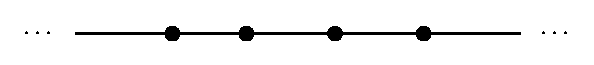
\includegraphics{unendldiam}
\end{center}
ist ein Baum von unendlichem Durchmesser. Hier ist eine Translation
ein Automorphismus ohne Fixpunkt und Fixkante.

\FOLG \label{folg_endpkt}
Jeder endliche Baum entsteht aus $\bullet$ durch wiederholtes
Anhängen von Endpunkten.

\DB Es sei $\GR$ ein Graph.
\begin{enumerate}
\item Ein Teilbaum $T\subset \GR$ heißt \emph{aufspannend}\index{aufspannender Baum}\index{Baum!aufspannend}
(oder auch \emph{Gerüst}\index{Gerüst}), wenn $E(T)=E(\GR)$ ist.
\item Jeder zusammenhängende Graph besitzt einen aufspannenden
Teilbaum.
\end{enumerate}
\bew
Es sei $T_0\subset \GR$ ein Teilbaum. Ist $E(T_0)\neq E(\GR)$,
so gibt es eine Kante $k\in K(\GR)$ mit
$\ini(k)\in E(T_0)$ und $\ter(k)\not\in E(T_0)$.
Dann ist $T' := T_0\cap\{k,\bar{k},\ter(k)\}$ ein Teilbaum von
$\GR$.\\
Ist $\GR$ endlich, so erhalten wir mit Induktion einen
Teilbaum $T$ mit $E(T)=E(\GR)$.\\
Falls $\GR$ nicht endlich ist, betrachte die Menge $\calT$ der
Teilbäume von $\GR$. Es ist $\calT\neq\emptyset$ und $\calT$
ist durch die Teilbaumrelation partiell geordnet.
Ist $T_1\subset T_2\subset \cdots$ eine austeigende Kette von
Teilbäumen, so ist $\bigcup_i T_i \in \calT$.
Nach dem Zornschen Lemma muss es also ein maximales Element
$T\in \calT$ geben.
Angenommen $E(T)\neq E(\GR)$. Dann könnte man wie im endlichen Fall
einen Baum $T'\supsetneq T$ konstruieren, im Widerspruch zur
Maximalität von $T$.
\qed

\DB \label{bem_geschlecht}
Sei $\GR$ ein endlicher zusammenhängender Graph.
Wir setzen
\begin{align*}
&e(\GR) := |E(\GR)|,\\
&k(\GR) := \frac{1}{2}|K(\GR)|.
\end{align*}
Das \emph{Geschlecht}\index{Geschlecht} von $\GR$ ist
\[
g(\GR) := k(\GR) - e(\GR) + 1.
\]
Das Geschlecht wird auch als \emph{zyklomatische Zahl}\index{zyklomatische Zahl (siehe Geschlecht)}
oder \emph{Betti-Zahl}\index{Betti-Zahl (siehe Geschlecht)}
bezeichnet.
Es gilt:
\begin{enumerate}
\item $g(\GR) \geq 0$.
\item $g(\GR) = 0$ genau dann, wenn $\GR$ ein Baum ist.
\end{enumerate}
\bew Ist $\GR$ ein Baum, so ist nach Folgerung \ref{folg_endpkt}
$g(\GR)=0$. Ist $\GR$ kein Baum, so sei $T$ ein aufspannender Baum
von $\GR$. Also ist $e(\GR)=e(T)$ und $k(\GR)>k(T)$ und damit
$g(\GR)>g(T)=0$.
\qed

\DB Sei $\GR$ ein Graph und $Z$ ein zusammenhängender Teilgraph.
Mit $\GR/Z$ bezeichnen
wir den folgenden Graphen
\begin{align*}
E(\GR/Z) &= ( E(\GR)-E(Z) )\cup\{z\},\\
K(\GR/Z) &= K(\GR)-K(Z),\\
I_{\GR/Z}(k) &= (\ini_{\GR/Z}(k),\ter_{\GR/Z}(k)), \quad k\in K(\GR/Z).
\end{align*}
mit
\[
\ini_{\GR/Z}(k) =
\left\{\begin{matrix}
\ini(k), & \ini(k)\not\in E(Z),\\
z, & \ini(k)\in E(Z)
\end{matrix}\right.
\quad
\text{ und }
\quad
\ter_{\GR/Z}(k) =
\left\{\begin{matrix}
\ter(k), & \ter(k)\not\in E(Z),\\
z, & \ter(k)\in E(Z)
\end{matrix}\right.
.
\]
\begin{center}
	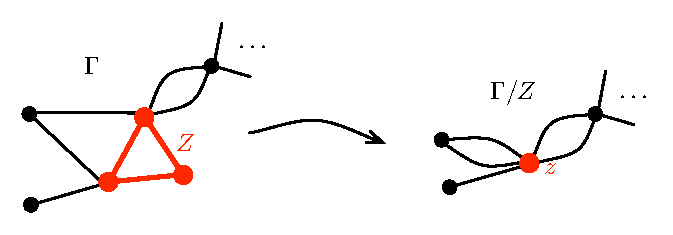
\includegraphics{GZ1}
\end{center}

\BSP Ist $Z$ das Gerüst von $\GR$, so erhalten wir
\begin{center}
%	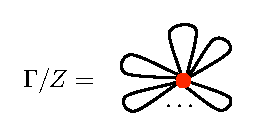
\includegraphics{GZ2}
\end{center}
mit $g(\GR)$ Kanten.

\DEF
Wir sagen, dass $\GR/Z$ aus $\GR$ durch \emph{Kontraktion}\index{Kontraktion}
von $Z$ entsteht.
Ist $Z$ nicht zusammenhängend, so wird $\GR/Z$ durch Kontraktion
jeder Zusammen\-hangskomponente von $Z$ definiert.

\BEM \label{bem_GZ}
Ist $\GR$ ein endlicher zusammenhängender Graph und $Z$ ein
Teilgraph, so gilt:
\begin{enumerate}
\item $g(\GR/Z) \leq g(\GR)$.
\item $g(\GR/Z) = g(\GR)$, falls $Z$ ein Teilbaum ist.
\end{enumerate}

\DEF Ein Graph, dessen Zusammenhangskomponenten Bäume sind,
heißt \emph{Wald}\index{Wald}.

\BEM Es sei $\GR$ ein zusammenhängender Graph und $Z$ ein Teilwald
von $\GR$. Dann ist $\GR/Z$ genau dann ein Baum, wenn $\GR$ ein
Baum ist.

\bew Ist $\GR$ endlich, so folgt die Behauptung aus Bemerkung
\ref{bem_GZ} und Bemerkung \ref{bem_geschlecht}.
Ist $\GR$ unendlich, so sei $\GR'$ ein endlicher zusammenhängender
Teilgraph von $\GR$. Dann ist $\GR'\cap Z$ ein endlicher Wald.
Also ist $\GR'$ ein Baum, genau dann wenn $\GR'\cap Z$ ein Baum
ist. Schöpfe nun $\GR$ durch endliche Teilgraphen aus.
\qed

